\section{Схема установки}

\begin{figure}[h]
	\begin{center}
		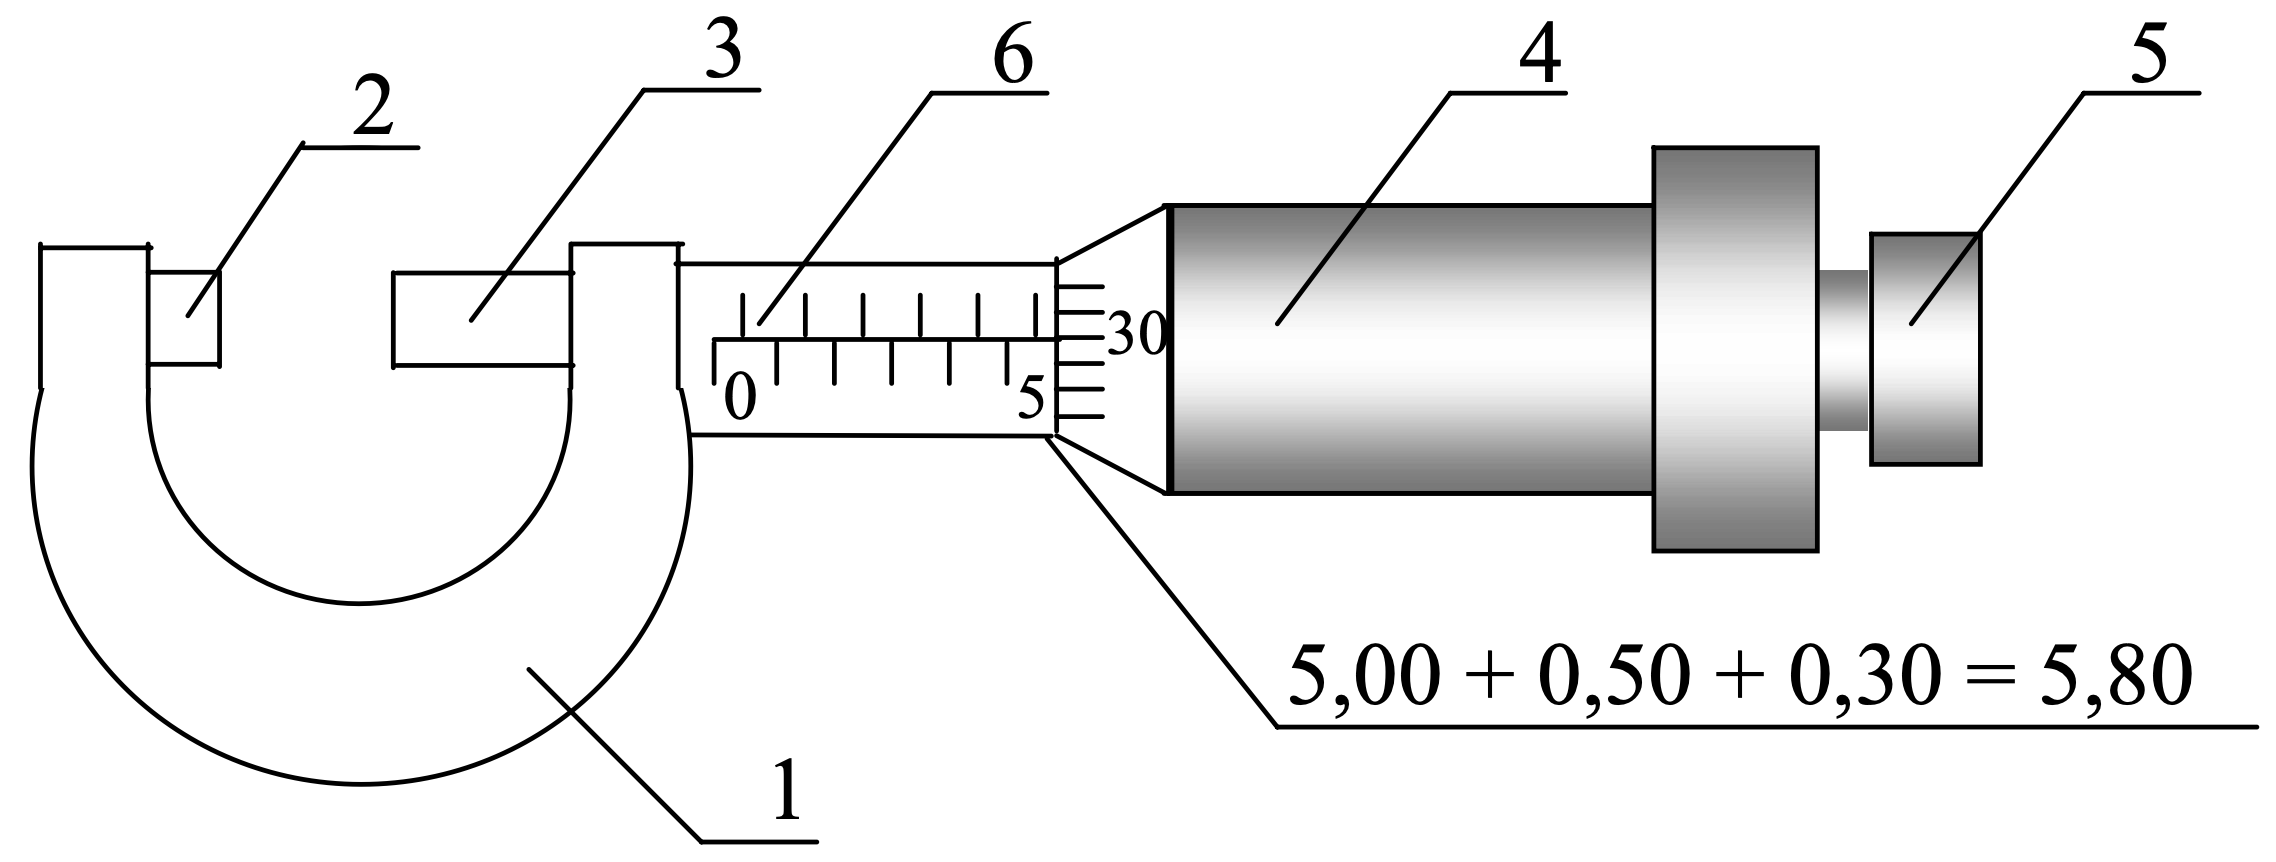
\includegraphics[width=0.7\textwidth]{pictures/PictureThree}
		\caption{Микрометр}\label{PicThree}
	\end{center}
\end{figure}

Устройство микрометра представлено на рисунке~\ref{PicThree}. Он состоит из скобы 1, в муфтах которой находятся упор 2 и микрометрический винт со стержнем 3. Цифрой 4 обозначена подвижная трубка, слева на которой располагается шкала. Вращение винта осуществляется движением головки 5. По шкале 6 измеряется число целых миллиметров.

\begin{figure}[h]
	\begin{center}
		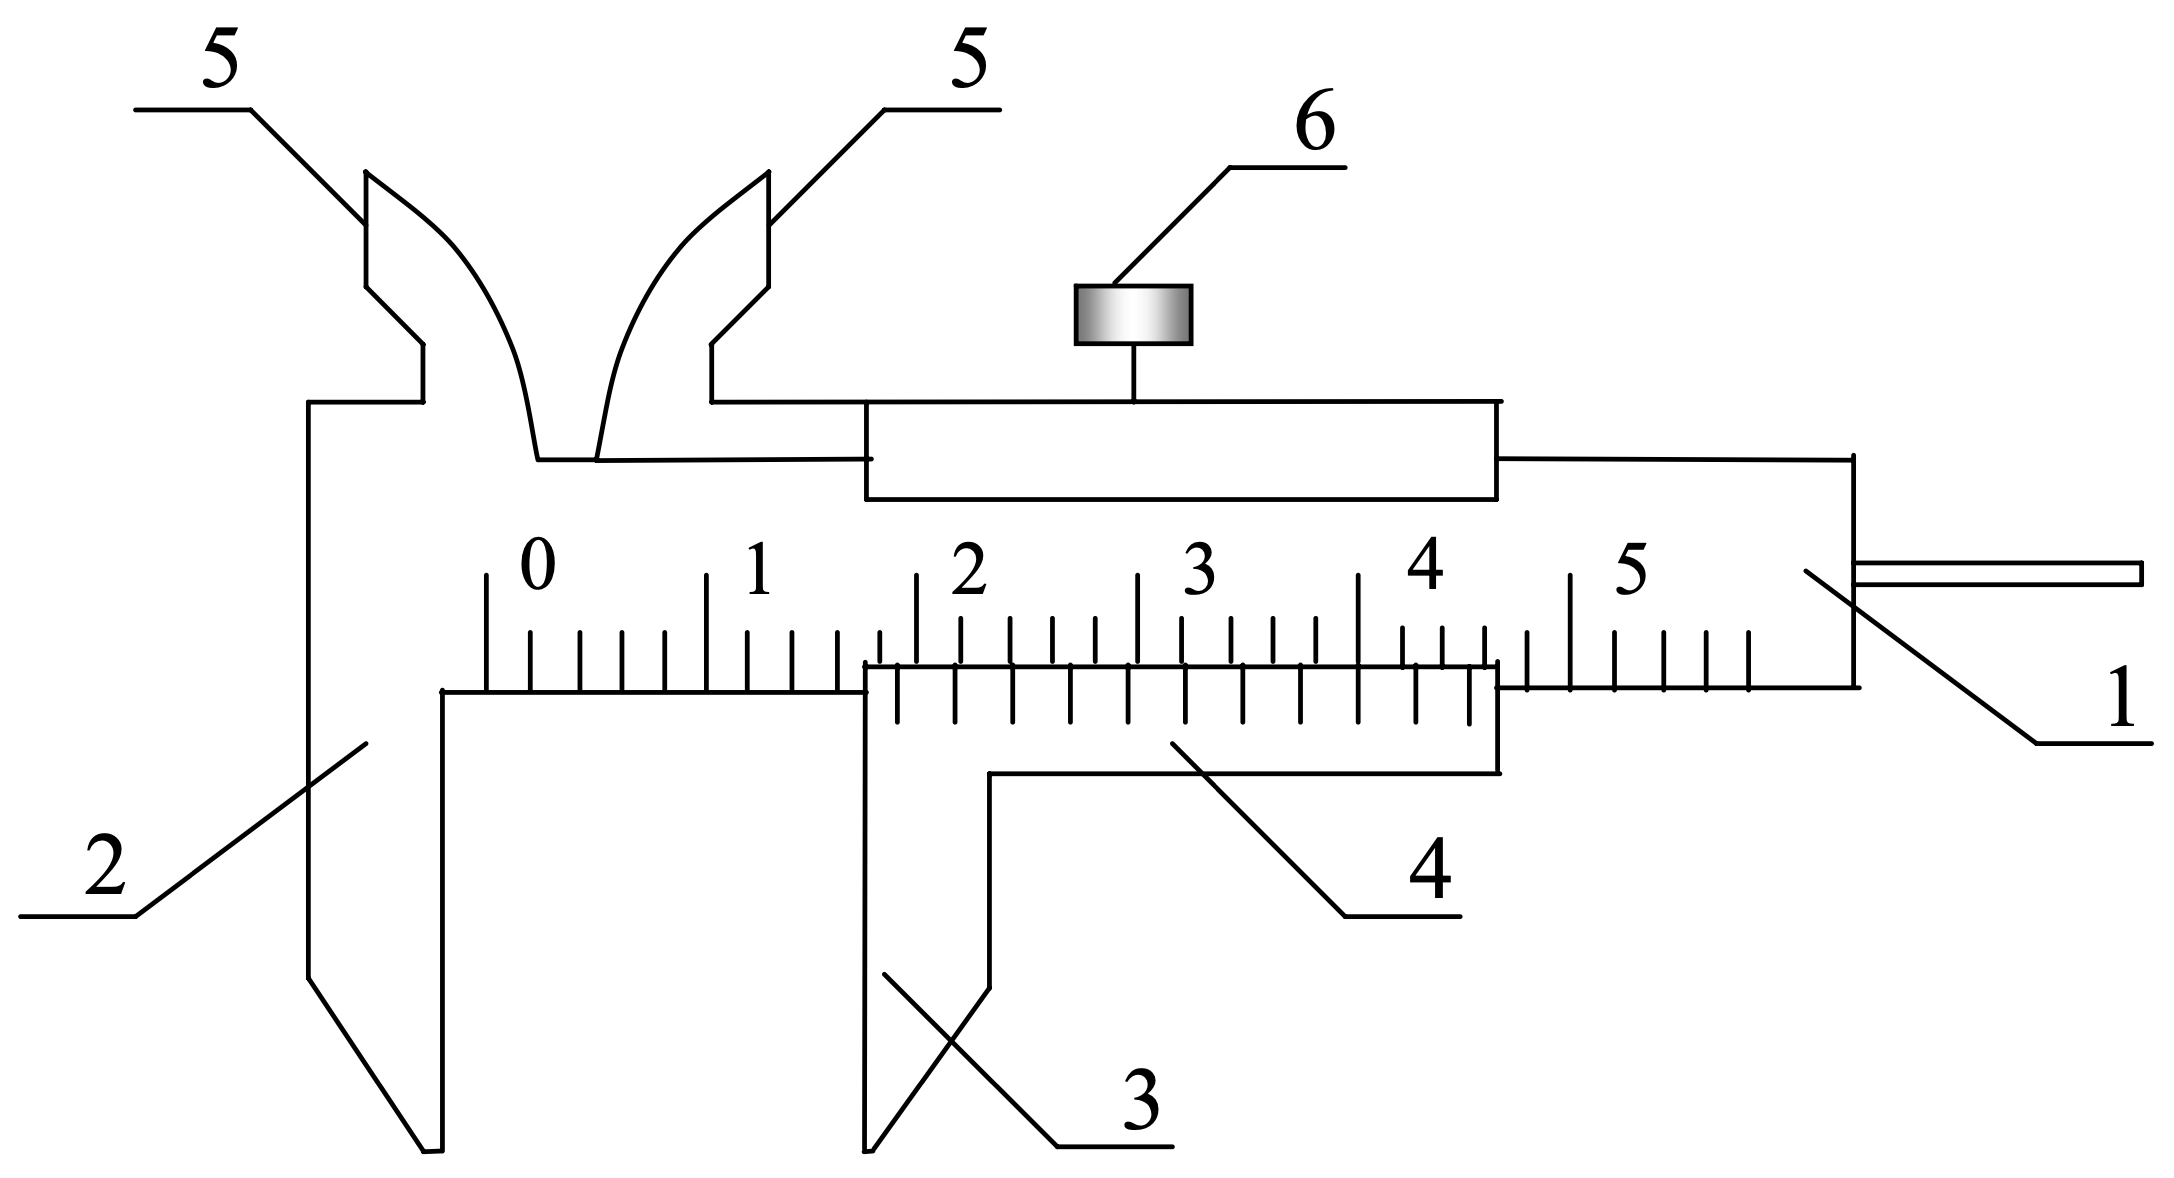
\includegraphics[width=0.7\textwidth]{pictures/PictureFour}
		\caption{Штангенциркуль}\label{PicFour}
	\end{center}
\end{figure}

На рисунке~\ref{PicFour} представлен штангенциркуль. Его основой является стальная миллиметровая линейка 1, снабжённая статичной ножкой 2 и подвижной ножкой 3. Подвижна ножка соединена с нониусом 4. Части 5 конструкции штангенциркуля используются для измерения внутренних размеров тел. Винт 6 предназначен для фиксации положения нониуса. 